\section{Machine learning}

Machine learning (ML) is a subgroup of artificial intelligence (AI), which encompasses a long range of computational models that learns from high quantities of data to classify and recognise patterns. The learning is either directed in a \textit{supervised} way with labeled data structures or in an \textit{unsupervised} way where the system aims to identify patterns without a predefined structure or truth. In both cases (supervised or unsupervised) the model is working to minimize a loss or cost function that captures the deviation of the predicted or generated output relative to the ground truth or input.\\

\noindent
Within the realm of microbiome research, ML models have been applied in several cases for the purpose of classification. ML have been developed for host phenotyping using the microbiome composition and bacterial species abundance as the only information and can successfully stratify patients based on their microbial signature \cite{Pasolli2016-pi,Statnikov2013-gz}. Some ML models also include functions for assessing feature importance on model performance, which have been used to identify discriminative bacterial strains that exacerbate a disease phenotype \cite{Pasolli2016-pi}. The features represent measurable or categorical units in the dataset, such as the abundance of bacterial species or whether the sample is from a control or case patient. Microbial features can be combined with other omics such as metabolomics, gene-expression or host clinical data to increase the models ability to differentiate phenotypes \cite{Zhou2019-nc}. The choice of ML method to use for each application largely depends on the data, method preference and importantly whether or not the data is complete with truth-labels to facilitate supervised learning of the model. Methods that have been used for supervised learning in microbiome studies are manyfold and include logistic regression, Linear Discriminant Analysis, support vector machines (SVMs), naive bayes classifiers and artificial neural networks \cite{Marcos-Zambrano2021-eg}. For one of the publications in this dissertation, we leveraged the Random Forest (RF) model.

\subsection{Random Forest}

The RF model is an ensemble of multiple decision trees in which the performance is evaluated based on pre-labelled data. Each individual tree in the RF makes a class prediction and the majority vote across all trees becomes the final prediction, thereby employing the “wisdom of the crowds” instead of relying on a single classifier. For a given training dataset with x number of observations characterized by y variables, the RF model constructs a prespecificied number of random decision trees (Figure \ref{fig:RF}). The randomness comes into play as the y-variables used to describe each observation are randomly sampled at each node in the decision trees.

\begin{figure}[H]
  \begin{center}
    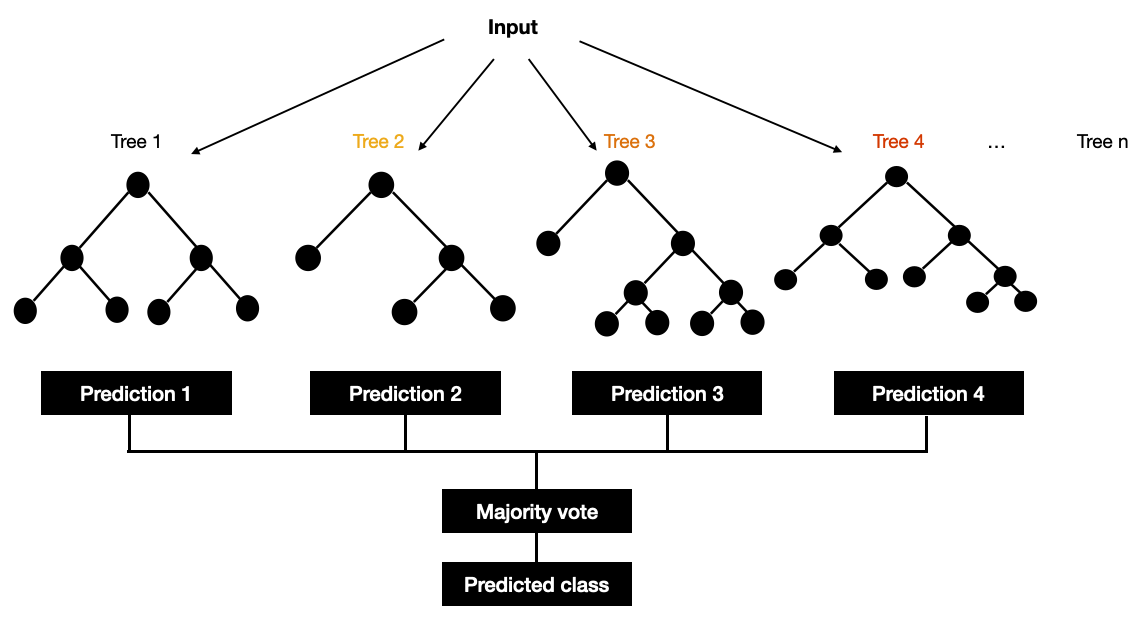
\includegraphics[scale=1, width=1\textwidth]{pictures/Random_forest.png}
  \end{center}
  \caption[VirusTimeline]{The Random Forest (RF) contains a predefined number of decision trees, which are randomly constructed resulting in n independent decision trees. A trained RF model works by receiving an input that is processed by each decision tree in the forest, which produces an independent prediction of the class based on the input. The final prediction is based on a majority vote across all trees to produce a final prediction.
  }
  \label{fig:RF}
\end{figure}

\noindent
The RF model is evaluated using a method called bagging as it randomly samples with replacements from the observations in the dataset. This also means that some observations are not sampled and therefore “bagged” in the out of bag (OOB) set, which can be used to test the accuracy of the final tree ensemble. Based on the OOB observations, an OOB-error is derived and provides an immediate estimate of the RF model's accuracy. When training other supervised ML methods like linear regression classifiers or SVMs that do not employ OOB, \textit{k}-fold cross validation (CV) is an ideal approach for testing the accuracy of the model during training and ensuring that the accuracy is calculated based on observations not used in estimating the parameters of the model. With CV, the observations are split into \textit{k} number of partitions; then the training is performed \textit{k} times using one partition of the observations as the test dataset and the rest as training data. To achieve a final estimate on whether the ML model generalizes to new observations, the most important estimate of accuracy should ideally be calculated based on an independent dataset. An overfitted model may produce good results on the training data set but underperform on real-world data points.

\subsection{Variational autoencoders}

One of the artificial neural network methods that has received increased attention is the autoencoder that has proven useful for capturing structures in high dimensional data with many features per observation such as single-cell RNA-seq and multi-omics data \cite{Ma2019-mp,Wang2021-ne}. Autoencoders are designed to receive an input and encode it into a compressed representation coined the latent representation, which can be decoded to reconstruct the input. The autoencoder is trained to minimize the difference between the original input and decoded output by minimizing a loss function that captures this difference numerically (Figure \ref{fig:encodedecode}).

\begin{figure}
  \begin{center}
    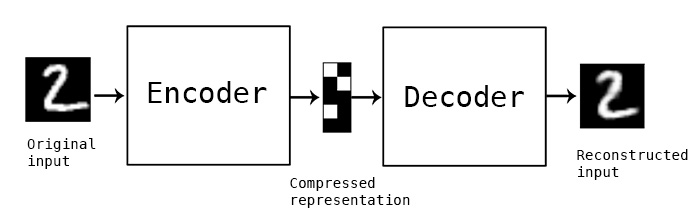
\includegraphics[scale=1, width=1\textwidth]{pictures/ML_autoencoder_schema.jpeg}
  \end{center}
  \caption[VirusTimeline]{A classic example of Autoencoders is the usage for reconstructing images. In the example depicted, the original input (image of a “2”) is encoded into a compressed representation and decoded into an output very similar to the original image. Illustration from: https://blog.keras.io/building-autoencoders-in-keras.html
  }
  \label{fig:encodedecode}
\end{figure}

\noindent
Autoencoders consist of a chain of artificial neural network (ANN) layers with a distinct architecture in which the first layer (that receives an input) has the same dimension of the last layer (which recreates the input). In the process of encoding a high-dimensional input $y$ into a low-dimensional compressed representation $z$, which can be decoded into an approximation of the original input $\hat{y}$ (Figure \ref{fig:VAE}), the network can capture important nonlinear structures in a dataset. The property for turning high-dimensional data into a low dimensional compressed representation $z$ makes the autoencoder a dimensionality reduction method as it learns to store all the relevant information in a few explanatory variables. An issue with the traditional autoencoder architecture is the fixation on encoding and decoding an input with as little loss of information as possible, which can lead to overfitting. If the autoencoder is overfitted, the encoder may map any data point to an arbitrarily small segment of the latent space $z$ as real numbers where the decoder can still recreate the input but the position in latent space is structurally meaningless. The autoencoders’ mapping of an input $y$ into the latent space $z$ can therefore become completely arbitrary. This would effectively make the autoencoder produce gibberish when exposed to new data points. In addition, arbitrary mapping of input into latent space makes it impossible to cluster the latent representation $z$ into anything meaningful if unrelated data points are positioned close in latent space.\\
\noindent
With Variational autoencoders (VAE), the training is performed using a regularization technique to avoid overfitting and enforce structure to the data points in latent space. The key is to ensure that data points that are close in the input space are also close in the latent space, which makes clustering of the latent space more feasible. To achieve this, the input $y$ is encoded as a Gaussian $\mathcal{N}(\mu, \sigma)$ distribution with a mean $\mu$ and standard deviation $\sigma$ by a function $E(y)$ \ref{fig:VAE}), instead of a low-dimensional data point. From the latent distribution $p(z)$, a latent representation $z$ is sampled and decoded into $\hat{y}$, which makes the VAE a generative model. 

\begin{figure}[H]
  \begin{center}
    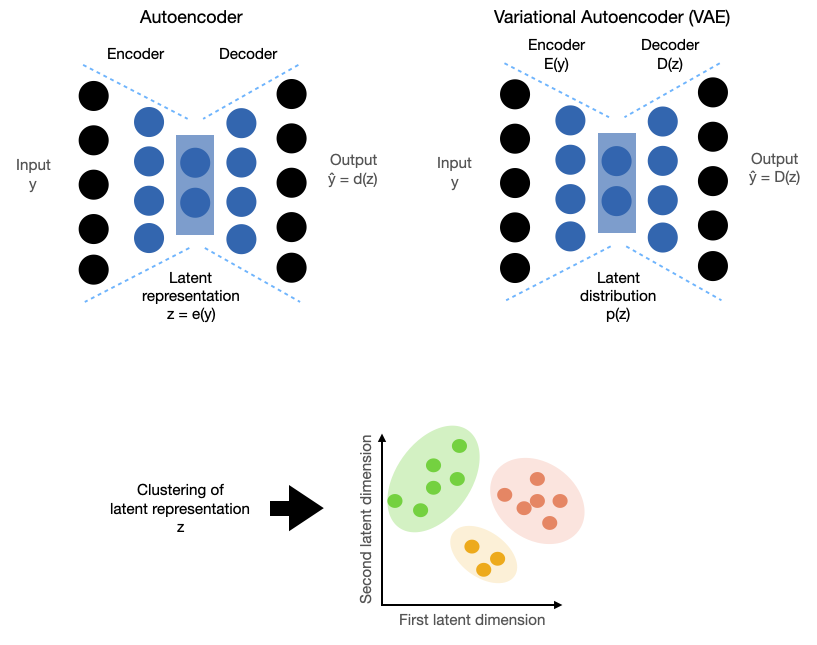
\includegraphics[scale=1, width=1\textwidth]{pictures/VAE.png}
  \end{center}
  \caption[VirusTimeline]{The Autoencoder and Variational Autoencoder (VAE) may have similar architectures as they both contain an input layer $y$ and output $\hat{y}$ layer with same dimensions, an encoder and decoder layer and a latent representation (center layer). However, the VAE encodes the input into a latent distribution $p(z)$ function that can be sampled from to reconstruct the input. Both methods can produce a latent representation $z$ for a group of high-dimensional data points that is more suitable for clustering and can be visualized in a lower dimensional space.
  }
  \label{fig:VAE}
\end{figure}

\noindent
For training the VAE, the loss function is composed of two terms \cite{Doersch2016-bo}; (1) a reconstruction error that represents the difference between the original input $y$ and the decoded output $\hat{y}$ and (2) a regularization term on the latent layer that enforces the encoder to return a gaussian distribution $\mathcal{N}$. The regularization term is expressed as the Kulback-Leibler (KL) divergence function that captures how well the encoded Gaussian distribution approximates a standard Gaussian distribution $\mathcal{N}(0,1)$ where $\mu$ is 0 and $\sigma$ is equal to 1. These two terms together make up The Evidence Lower BOund (ELBO) function also described as the variational lower bound. The ELBO can either be represented as the expected negative log likelihood plus the KL divergence, where the ELBO loss function is minimized during training of the VAE.

\begin{equation}
ELBO(y) = -\mathbb{E}_{E}[log(p(y|z))] - D_{KL}(E(y) \Vert p(z))
\end{equation}

\noindent
Or as an expression where the ELBO is maximized by minimizing the KL divergence while maximizing the expected log-likelihood.

\begin{equation}
ELBO(y) = \mathbb{E}_{E}[log(p(y|z))] - D_{KL}(E(y) \Vert p(z))
\end{equation}

\noindent
Ultimately, what we want to achieve using a VAE is to map similar values closely in the latent space. Compared to an ordinary autoencoder trained to decode arbritary data points into near exact recreations of the input, in the VAE the decoder samples from encoded Gaussian distributions of the input, which results in similar recreations of the input instead of near exact. The VAE’s capacity for encoding high-dimensional observations into meaningful low-dimensional numeric vectors without any prior labeling of observations makes it an unsupervised and powerful method for dimensionality reduction and clustering. Biological samples from patients or natural environments are characterized today with thousands of features produced by multi-omics, thus the VAE is getting more recognised as an appropriate tool for differentiating anything from cell types to human pathologies.  
